\documentclass[border=3pt,tikz]{standalone}
\usepackage[utf8]{vietnam}
\usetikzlibrary{calc,angles,intersections,shapes.geometric,arrows,decorations.markings,arrows.meta,patterns.meta,patterns}
\usepackage{tikz-3dplot,pgfplots}
\pgfplotsset{compat=1.15}
\usepgfplotslibrary{polar}
\usepackage{amsmath}
\begin{document}
	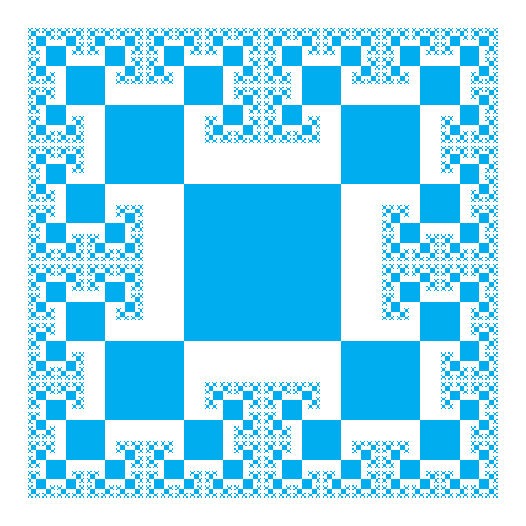
\begin{tikzpicture}
		\newcommand{\hv}[3][]{
			\ifnum#2>0
			\path[#1] (-1,-1) rectangle (1,1);
			\pgfmathtruncatemacro{\k}{#2-1}
			\foreach \i in {0,1,2,3}{
				\pgfmathtruncatemacro{\goc}{90*\i+45-#3}
				\ifnum\goc=180\else\ifnum\goc=-180\else
				\pgfmathtruncatemacro{\g}{90*\i+45}
				\begin{scope}[shift={(\g:{1.5*sqrt(2)})},scale=1/2]
					\hv[#1]{\k}{\g}
				\end{scope}
				\fi\fi
			}
			\fi
		}
		\hv[fill=cyan]{8}{0}
	\end{tikzpicture}

	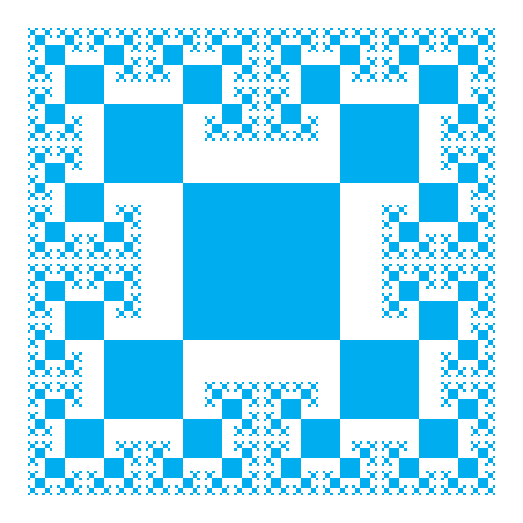
\begin{tikzpicture}
		\newcommand{\hv}[3][]{
			\ifnum#2>0
			\path[#1] (-1,-1) rectangle (1,1);
			\pgfmathtruncatemacro{\k}{#2-1}
			\foreach \i in {0,1,2,3}{
				\pgfmathparse{abs(90*\i+45-#3)!=180}
				\ifnum\pgfmathresult=1
				\pgfmathsetmacro{\g}{90*\i+45}
				\begin{scope}[shift={(\g:{1.5*sqrt(2)})},scale=1/2]
					\hv[#1]{\k}{\g}
				\end{scope}
				\fi
			}
			\fi
		}
		\hv[fill=cyan]{7}{0}
	\end{tikzpicture}
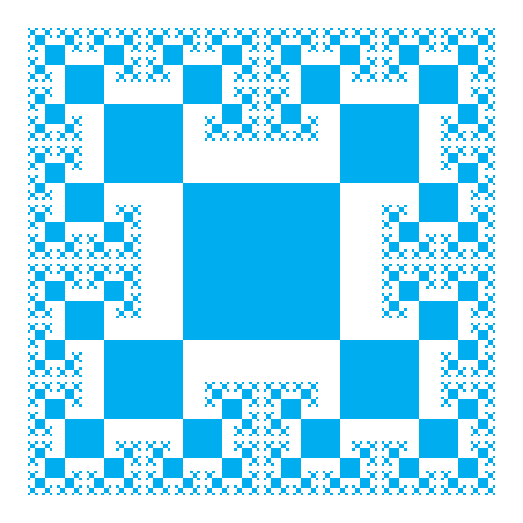
\begin{tikzpicture}
	\newcommand{\hv}[3][]{
		\ifnum#2>0
		\path[#1] (-1,-1) rectangle (1,1);
		\pgfmathtruncatemacro{\k}{#2-1}
		\foreach \i in {0,1,2,3}{
			\pgfmathparse{(90*\i+45-#3)-180 && (90*\i+45-#3)+180}
			\ifnum\pgfmathresult=1
			\pgfmathsetmacro{\g}{90*\i+45}
			\begin{scope}[shift={(\g:{1.5*sqrt(2)})},scale=1/2]
				\hv[#1]{\k}{\g}
			\end{scope}
			\fi
		}
		\fi
	}
	\hv[fill=cyan]{7}{0}
\end{tikzpicture}
\end{document}